\documentclass[a4paper,11pt]{article}
\usepackage{xcolor}
\usepackage{tikz}
\usetikzlibrary{shapes.arrows,arrows.meta}
\begin{document}
\begin{figure}[h!]
  \begin{center}
  \scalebox{0.2}{
    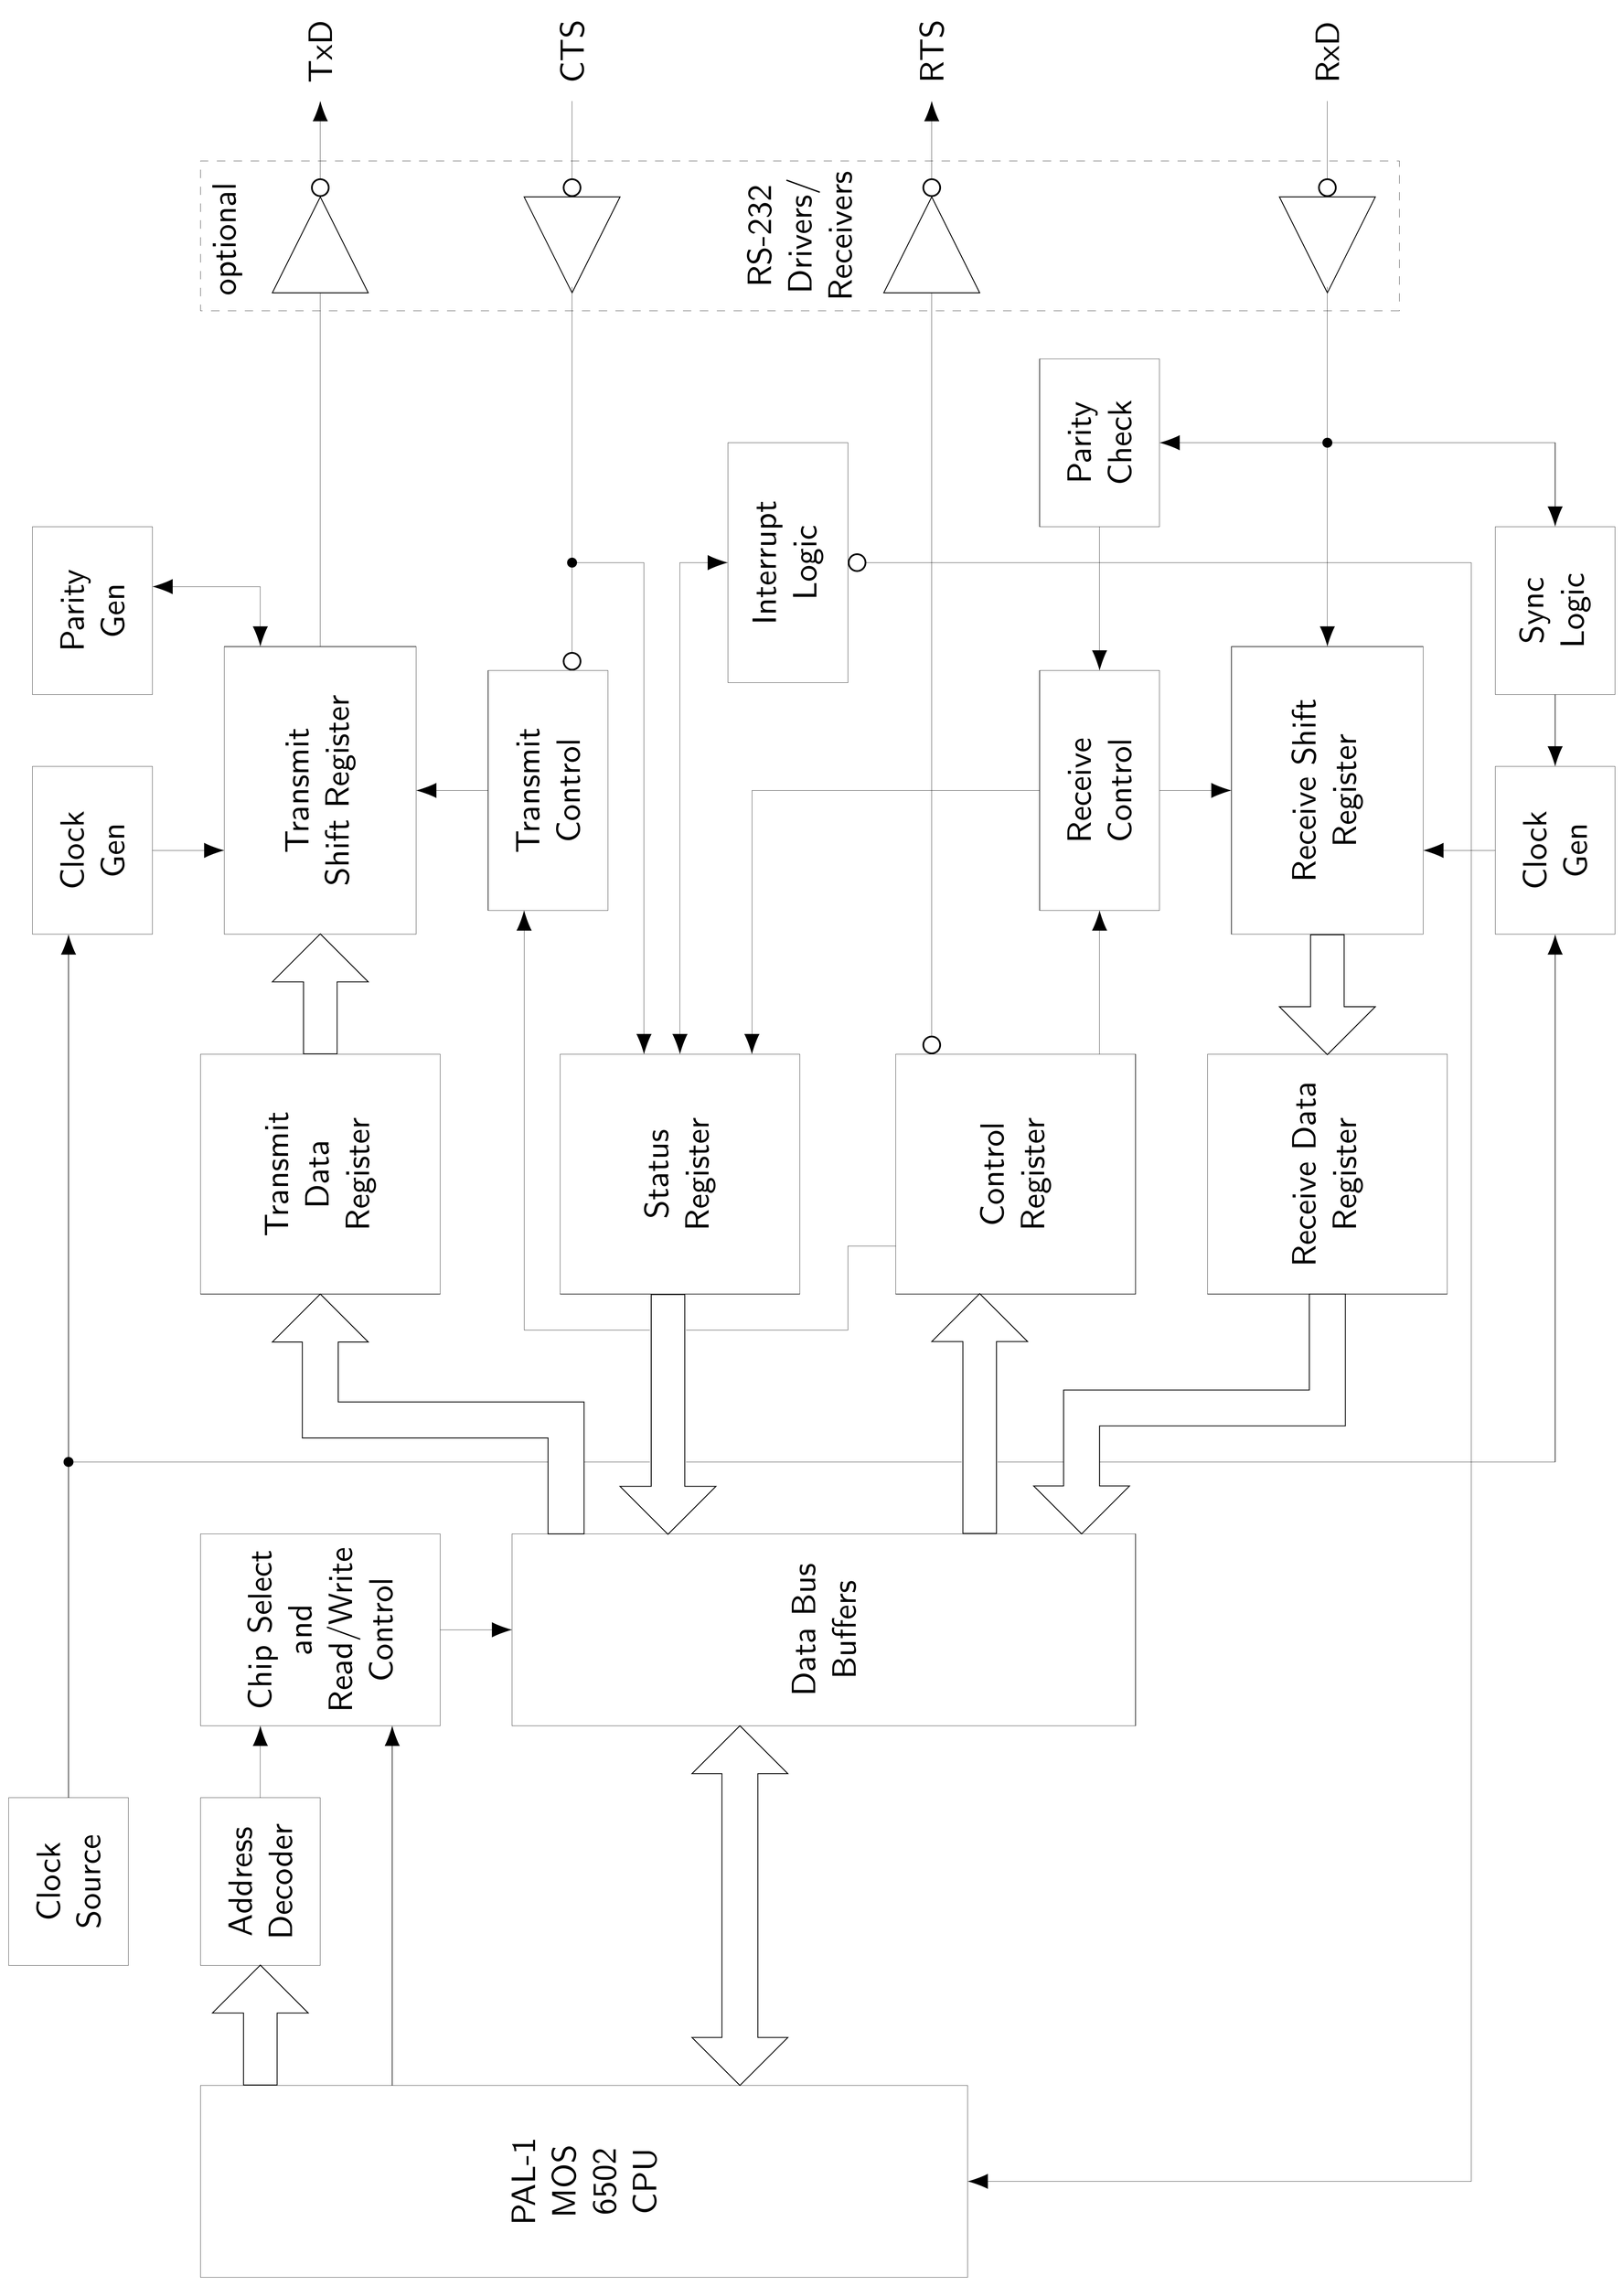
\begin{tikzpicture}[font=\sffamily,rotate=90,transform shape]
    	\draw (20, 10) rectangle ++(10,10) node[pos=.5,scale=4,text width=2cm,align=center] {Receive Data Register};	
    	\draw (20, 23) rectangle ++(10,10) node[pos=.5,scale=4,text width=2cm,align=center] {Control Register};	
    	\draw (20, 37) rectangle ++(10,10) node[pos=.5,scale=4,text width=2cm,align=center] {Status Register};
    	\draw (20, 52) rectangle ++(10,10) node[pos=.5,scale=4,text width=2cm,align=center] {Transmit Data Register};		
	\draw (35,11) rectangle ++(12,8) node[pos=.5,scale=4,text width=2cm,align=center] {Receive Shift  Register};
	\draw (35,53) rectangle ++(12,8) node[pos=.5,scale=4,text width=2cm,align=center] {Transmit Shift  Register};
	\draw(35,3) rectangle ++(7,5) node[pos=0.5,scale=4,text width=1.5cm,align=center] {Clock Gen};
	\draw(45,3) rectangle ++(7,5) node[pos=0.5,scale=4,text width=1.5cm,align=center] {Sync Logic};
	\draw(35,64) rectangle ++(7,5) node[pos=0.5,scale=4,text width=1.5cm,align=center] {Clock Gen};
	\draw(45,64) rectangle ++(7,5) node[pos=0.5,scale=4,text width=1.5cm,align=center] {Parity Gen};
	\draw(36,22) rectangle ++(10,5) node[pos=.5,scale=4,text width=2cm,align=center] {Receive Control};
	\draw(36,45) rectangle ++(10,5) node[pos=.5,scale=4,text width=2cm,align=center] {Transmit Control};
	\draw(52,22) rectangle ++(7,5) node[pos=0.5,scale=4,text width=1.5cm,align=center] {Parity Check};
	\draw(45.5,35) rectangle ++(10,5) node[pos=0.5,scale=4,text width=1.5cm,align=center] {Interrupt Logic};
	\draw(2,23) rectangle ++(8,26) node[pos=0.5,scale=4,text width=1.5cm,align=center] {Data Bus Buffers};
	\draw(2,52) rectangle ++(8,10) node[pos=0.5,scale=4,text width=2.5cm,align=center] {Chip Select \\and\\Read/Write Control};
	\draw(-8,57) rectangle ++(7,5) node[pos=0.5,scale=4,text width=1.5cm,align=center] {Address Decoder};
	\draw(-8,65) rectangle ++(7,5) node[pos=0.5,scale=4,text width=1.5cm,align=center] {Clock Source};
	\draw(-21,30) rectangle ++(8,32) node[pos=0.5,scale=4,text width=1.5cm,align=center] {PAL-1 MOS 6502 CPU};
	\draw[dash pattern=on 10pt off 10pt](61,12) rectangle ++(6.25,50)
			node[pos=0.5,scale=4,text width=1.5cm,align=center] {RS-232 Drivers/ Receivers};
	
	\draw[-{Latex[scale=5]}](62,15) -- ++(-15,0);
	\draw[arrows={Latex[scale=5]-Latex[scale=5]}](52,5.5) -- ++(3.5,0) -- ++(0,16.5);
	\draw[arrows={Latex[scale=5]-Latex[scale=5]}](50.5,40) -- ++(0,2) -- ++(-20.5,0);
	\draw[arrows={Latex[scale=5]-Latex[scale=5]}](49.50,64) -- ++(0,-4.5) -- ++(-2.5,0);
	\draw[-{Latex[scale=5]}](38.5,8) -- ++(0,3);
	\draw[-{Latex[scale=5]}](41,50) -- ++(0,3);
	\draw[-{Latex[scale=5]}](45,5.5) -- ++(-3,0);
	\draw[-{Latex[scale=5]}](41,22) -- ++(0,-3);
	\draw[-{Latex[scale=5]}](38.5,64) -- ++(0,-3);
	\draw[-{Latex[scale=5]}](6,52) -- ++(0,-3);
	\draw[-{Latex[scale=5]}](-1,59.5) -- ++(3,0);
	\draw[-{Latex[scale=5]}](52,24.5) -- ++(-6,0);
	\draw[-{Latex[scale=5]}](30,24.5) -- ++(6,0);
	\draw[-{Latex[scale=5]}](-13,54) -- ++(15,0);
	\draw[-{Latex[scale=5]}](41,27) -- ++(0,12) -- ++(-11,0);
	\draw[-{Latex[scale=5]}](50.5,46.5) -- ++(0,-3) -- ++(-20.5,0);		
	\draw(22,33) -- ++(0,2) -- ++(-3.5,0) -- ++(0,6.75);
	\draw[-{Latex[scale=5]}](18.5,43.25) -- ++(0,5.25) -- ++(17.5,0);
	\draw[-{Latex[scale=5]}](-1,67.5) -- ++(36,0);
	\draw(47,57) -- ++(14.75,0);
	\draw(13,67.5) -- ++(0,-20);
	\draw(13,46) -- ++(0,-2.75);				
	\draw(13,41.75) -- ++(0,-11.5);	
	\draw(13,28.75) -- ++(0,-2.75);		
	\draw[-{Latex[scale=5]}](13,24.5) -- ++(0,-19) -- ++(22,0);
	
	\draw[fill=black] (55.5,15) circle (2mm);
	\draw[fill=black] (50.5,46.5) circle (2mm);
	\draw[fill=black] (13,67.5) circle (2mm);
		
	\draw[{Circle[open,scale=6,line width=2]}-](30,31.5) -- ++(31.75,0);
	\draw[arrows={Circle[open,scale=6,line width=2]-Latex[scale=5]}](50.5,35) -- ++(0,-26) -- 
			++(-67.5,0) -- ++(0,21);
	\draw[{Circle[open,scale=6,line width=2]}-](46,46.5) -- ++(16,0);
	
	\draw (35,15) node [draw,single arrow, minimum height=5cm, minimum width=4cm,
	                             anchor=west,line width=1,rotate=180] {};
	\draw (30,57) node [draw,single arrow, minimum height=5cm, minimum width=4cm,
	                             anchor=west,line width=1] {};
	\draw (10,29.5) node [draw,single arrow, minimum height=10cm, minimum width=4cm,
	                             anchor=west,line width=1] {};
	\draw (20,42.5) node [draw,single arrow, minimum height=10cm, minimum width=4cm,
	                             anchor=west,line width=1,rotate=180] {};
	\draw (-13,59.5) node [draw,single arrow, minimum height=5cm, minimum width=4cm,
	                             anchor=west,line width=1] {};
	                             
	\draw[line width=1](10,46) -- ++(5.5,0) -- ++(0,10.25) -- ++(2.5,0) -- ++(0,-1.25) -- ++(2,2) -- 
			++(-2,2) -- ++(0,-1.25) -- ++(-4,0) -- ++(0,-10.25) -- ++(-4,0) -- cycle;
	\draw[line width=1](20,14.25) -- ++(-5.5,0) -- ++(0,10.25) -- ++(-2.5,0) -- ++(0,-1.25) -- ++(-2,2) --
			++(2,2) -- ++(0,-1.25) -- ++(4,0) -- ++(0,-10.25) -- ++(4,0) -- cycle;
	\draw[line width=1](-13,39.5) -- ++(2,2) -- ++(0,-1.25) -- ++(11,0) -- ++(0,1.25) -- ++(2,-2) --
			++(-2,-2) -- ++(0,1.25) -- ++(-11,0) -- ++(0,-1.25) -- cycle;
			
	\draw[line width=1](61.75,46.5) -- ++(4,2) -- ++(0,-4) -- cycle;
	\draw[{Circle[open,scale=6,line width=2]}-](65.75,46.5) -- ++(4,0);
	\draw[line width=1](61.75,15) -- ++(4,2) -- ++(0,-4) -- cycle;
	\draw[{Circle[open,scale=6,line width=2]}-](65.75,15) -- ++(4,0);
	
	\draw[line width=1](61.75,59) -- ++(4,-2) -- ++(-4,-2) -- cycle;
	\draw[arrows={Circle[open,scale=6,line width=2]-Latex[scale=5]}](65.75,57) -- ++(4,0);
	\draw[line width=1](61.75,33.5) -- ++(4,-2) -- ++(-4,-2) -- cycle;
	\draw[arrows={Circle[open,scale=6,line width=2]-Latex[scale=5]}](65.75,31.5) -- ++(4,0);

	\node[anchor=west,scale=4] at (70,57) {TxD};
	\node[anchor=west,scale=4] at (70,46.5) {CTS};
	\node[anchor=west,scale=4] at (70,31.5) {RTS};
	\node[anchor=west,scale=4] at (70,15) {RxD};
	\node[anchor=north,scale=4] at (64,62) {optional};
    \end{tikzpicture}
    }
    \caption{PAL-1 Serial Interface Adapter block diagram.}
    \label{sec:blockdiagram}
  \end{center}
\end{figure}
\end{document} 



